\documentclass[11pt,english]{article}

\usepackage[utf8]{inputenc}
\usepackage[T1]{fontenc}

\usepackage[
  margin=1.3in,
  headheight=14pt]{geometry}


\usepackage{mathpazo}
\usepackage{graphicx}
\usepackage{marginnote}
\usepackage{parskip}
\usepackage{microtype}
\usepackage{babel}
\usepackage{setspace}
\usepackage{lastpage}
\usepackage{fancyhdr}
\pagestyle{fancy}
\fancyhf{}
\lhead{Nathaniel Stemen}
\rhead{Advanced Quantum Theory}
\rfoot{\thepage/\pageref{LastPage}}
\usepackage{varioref}
\usepackage[dvipsnames]{xcolor}
\usepackage[linktocpage]{hyperref}
\hypersetup{
  linktoc=all,
  colorlinks=true,
  linkcolor=MidnightBlue,
  filecolor=RubineRed,
  urlcolor=Bittersweet,
  citecolor=Fuchsia,
}
\usepackage{physics}
\usepackage{mathtools}
\usepackage{float}
\usepackage{titletoc}
\usepackage{natbib}
\bibliographystyle{unsrtnat}
\usepackage[nottoc]{tocbibind}
\usepackage[noabbrev]{cleveref}
\usepackage{amsthm}
\theoremstyle{definition}
\newtheorem{definition}{Definition}[section]
\newtheorem{example}{Example}[section]

\newcommand{\twonorm}[1][\rho]{c_{2,B} (#1)}
\newcommand{\twonormE}[1][\rho]{c_{2,B}}
\newcommand{\dephase}{\mathcal{D}_B}
\newcommand{\iu}{\mathrm{i}\mkern1mu}
\newcommand{\e}{\mathrm{e}}


\titlecontents{section}[1.8pc]
  {\addvspace{3pt}\bfseries}
  {\contentslabel[\thecontentslabel]{1.8pc}}
  {}
  {\quad\thecontentspage}

\titlecontents{subsection}[1.8pc]
  {\addvspace{1pt}\small}
  {\thecontentslabel\enspace{}}
  {}
  {\quad\thecontentspage}

\titlecontents{subsubsection}[3.2pc]
  {\addvspace{1pt}\small}
  {\thecontentslabel\enspace{}}
  {}
  {\quad\thecontentspage}

\begin{document}

\begin{titlepage}
	\newcommand{\HRule}{\rule{\linewidth}{0.5mm}}

	\begin{center}

		\textsc{\LARGE University of Waterloo}\\[1.5cm]

		\textsc{\large AMATH 673 --- Advanced Quantum Theory}\\[0.75cm]

		\HRule{}\\[0.4cm]

		{\huge\bfseries Final Project}\\[0.15cm]

		\HRule{}\\[1cm]

		{\large
		\textbf{Name:} Nathaniel Stemen (20906566)\hspace{\fill} \textbf{Due:} December 21, 2020 \\
		\textbf{Email:} \href{mailto:nate.stemen@uwaterloo.ca}{\texttt{nate.stemen@uwaterloo.ca}} \hspace{\fill} \textbf{Professor:} Achim Kempf
		}

		\vfill
		
\includegraphics[width=0.8\textwidth]{uwlogo.jpg}\\[1cm]
	\end{center}
\end{titlepage}

\begingroup
\colorlet{darkblue}{MidnightBlue!10!black}
\hypersetup{linkcolor=darkblue}
\tableofcontents
\endgroup

\setstretch{1.1}

\vspace{0.5cm}
This is a summary/exposition of the article titled \emph{The Dynamics of Entropies at the Onset of Interactions} by~\citeauthor{dynamic-entropies}\marginnote{\footnotesize{Article can be found on the \href{https://arxiv.org/abs/2004.02829}{arXiv}.}} and was completed as a final project for AMATH 673 Advanced Quantum Theory.

\section{Background}
To begin, we first motivate the studies undertaken in~\cite{dynamic-entropies} as well as review some of the fundamental concepts that we will build upon.

\subsection{Motivation}

The theory of quantum mechanics has barely been around for a century, but it has managed to sew it's way into the core modern life; from lasers to Magnetic Resonance Imaging, quantum mechanics is here to stay. Not only that, but it has managed to become one of the most well tested theories in scientific history. With success seemingly around every corner, there's still a major advanced we haven't cracked: quantum computing. Since the first talk of quantum computers in the 1980's scientists have been hard at work bringing this technology to fruition. One of the main battles with such finnicky little beasts is coherence. Classical bits are robust against measurement and being dropped on the ground, but don't dare look at a quantum bit or it might have an identity crisis!

Coherence has been studied since the early days of quantum mechanics, and our continued inability to tame it in the lab indicates there's more to understand. When faced with such a situation, it is helpful to look back at moments in history that we can draw similarities to.

When physicists, mathematicians, and natural philosophers\footnote{Perhaps what they would have called themselves?} first studied the dynamics of colliding objects, there were perhaps three major motivating factors:
\begin{enumerate}
	\item it's an interesting problem in it's own right
	\item developing an understanding of the problem can help kickstart technologies harnessing a newfound understanding
	\item understanding a simplified problem is often good stepping stone to developing an understanding of a more complicated one
\end{enumerate}
Even though we might today consider the collision of physical bodies to be a relatively simple problem, there are many ways to look at this problem, and one of the most insightful is to think about the exchange of momenta. Now this varies depending on the elasticity of the collision, but understanding how two objects ``exchange'' momentum allows us to figure out what's going on. The particularly insightful thing here is that we're viewing a system as possessing momentum, which then during the collision, exchanges that property with another object before flying apart, or sticking together. With this framework we can build models of how bodies exchange momenta, what the rules of exchange are, and what exchanges are possible.

We do this with quantum bodies as well; usually motivated by the classical intuition. But, can we build theories where the thing being exchanged and swapped around \emph{is} coherence? Are there rules for the exchange of coherence between quantum bodies? If we could understand this, we might find ways to help tame \textbf{decoherence} or take advantage of \textbf{entanglement}. That's where resource theories come in to play.

\begin{figure}[h!]
	\begin{center}
		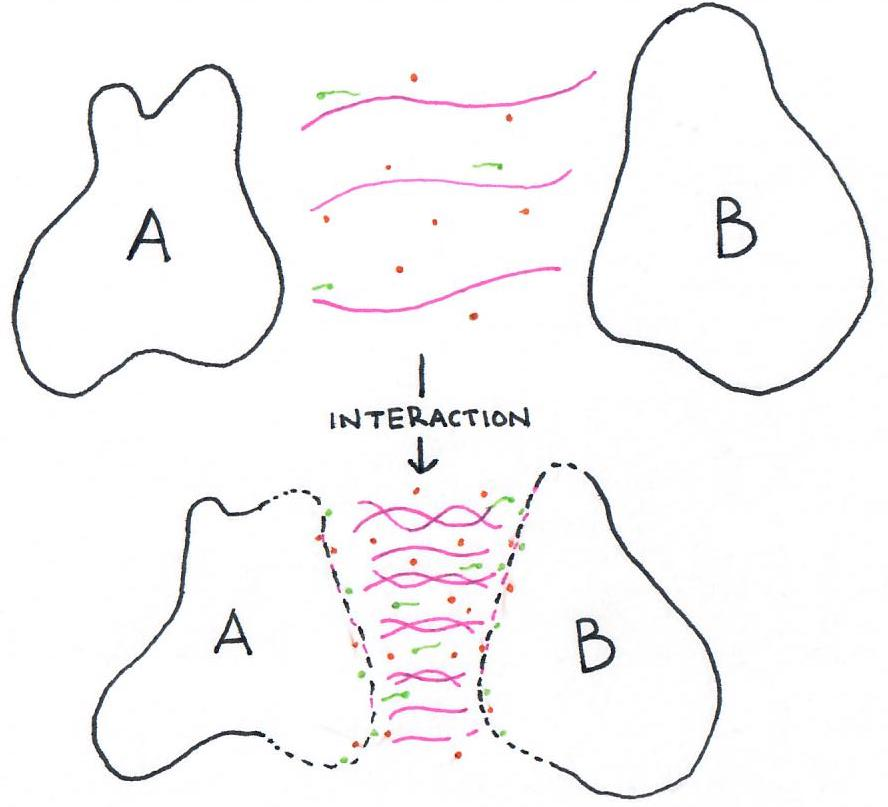
\includegraphics[width=0.5\textwidth]{interaction.jpeg}
		\caption{Two interacting systems}\label{fig:interacting-systems}
	\end{center}
\end{figure}


\subsection{Resource Theories}
When thinking of goods and the exchange of them, it's easy to think of economics, but this idea can be much more powerful as alluded to above. Resource theory is a branch of mathematics that allows us to dissect resources, and in particular their exchange and even the processes of change where one resource might turn into another (maybe we can turn coherence into entanglement?).

These general mathematical theories have been constructed~\cite{mathematical-resources,resource-theory} for studying anything from chemistry to economics. While the formal constructions are quite complicated using the language of category theory and ``symmetric monoidal categories'', the ideas are quite simple. The na\"\i ve questions we might want to ask are
\begin{itemize}
	\item how do resources change during allowed processes?
	\item what \emph{are} the allowed processes?
\end{itemize}
Or, put differently, what are the dynamics of our resources? These questions are encapsulated by category theory because of the way arrows (changes) and composition of arrows is the language of categories.

Quantum resource theories have also been developed with both coherence and entanglement as the star in~\cite{quantum-resources}. This means that we are taking coherence and entanglement as resources, and using these theories we can study how they change and are exchanged during interactions.

\subsection{Density Matrices}\label{sec:density-matrices}
Just briefly let's recall some facts about the density matrix that will be helpful in understanding this paper.
\begin{definition}
	A \textbf{density matrix} is a matrix of the form
	\begin{equation*}
		\rho = \sum_n p_n\ketbra{\psi_n}
	\end{equation*}
	where $p_n\in[0,1]$ are probabilities the mixed state $\rho$ is in the pure state $\ket{\psi_n}$ where the states $\{\ket{\psi_n}\}$ form a basis for our (finite dimensional) Hilbert space $\mathcal{H}$.
\end{definition}
The operator/matrix $\rho$ as defined above will always be positive semi-definite\footnote{$\bra{\phi}\rho\ket{\phi}\geq 0$ for all $\ket{\phi}\in\mathcal{H}$.}, Hermitian\footnote{$\rho^\dagger = \rho$.}, and have trace equal to 1\footnote{$\tr\rho = 1$.}. These three properties follow immediately from the above definition, along with the fact that the $p_n$ are probabilities and hence must sum to 1. Lastly recall that if we have an observable $\hat{A}$, then the expectation value with respect to a mixed state $\rho$ is given by $\overline{A} = \tr(\rho\hat{A})$.

\subsection{Entropy}
The paper is called ``The dynamics of entropies at the onset of interactions'', so it's probably best if we have a good understanding of what the authors mean by entropy.

Let's start with an arbitrary mixed state $\rho$. Because $\rho$ has trace 1, we know $\tr\rho^2\leq 1$ with equality holding if and only if $\rho$ is not in fact mixed, but a pure state $\rho = \ketbra{\psi}$. With this we can define a simple notion of ``purity'' by $\gamma = \tr\rho^2$. If $\rho$ represents an $n$ dimensional system, then $\gamma$ must fall in the range $\gamma\in\qty[\frac{1}{n}, 1]$ where the lowest values represent states that are more mixed, and higher values correspond to states that are more pure.

A more sophisticated measure of purity or mixedness coming from (classical) information theory would be the von Neumann entropy:
\begin{equation*}
	S(\rho)\coloneqq -\tr(\rho\ln\rho).
\end{equation*}
This measure does have the advantage of having an information theoretic backing, but in practice it is much harder to work with and calculate because of the logarithm.

Finally, there is one more notion we must introduce which is used in the paper. That of $n$-R\'enyi entropies, which can be defined as follows.
\begin{equation*}
	H_{n, B}(\rho)\coloneqq \frac{1}{1-n}\log(\tr_B\qty[\qty(\tr_A \rho)^n]) = \frac{1}{1-n}\log(\sum_i\lambda_i^n)
\end{equation*}
Where $\lambda_i$ are the eigenvalues of $\rho$. While it seems these entropies are not as frequently used, they provide a unifying framework for common entropies one does care about. In fact we have the max-entropy when $n = 0$, the min-entropy when $n\to\infty$, and the von Neumann entropy when $n \to 1$.


\section{Main Results}
We start off with a simple calculation of the 2-norm coherence, and then use this to study a two level quantum system.

\subsection{2-Norm Coherence}
Let's start with showing the 2-norm coherence $\twonorm{}$ is the sum of the off diagonal elements squared of $\rho$.
To start, let's calculate the effect of the identity minus the dephasing operator $\dephase$ on our mixed state $\rho$.
\begin{equation*}
	\qty(\mathbb{1} - \dephase)\rho = \mqty[\rho_{11} & \rho_{12} & \cdots & \rho_{1d} \\ \rho_{21} & \rho_{22} & & \\ \vdots & & \ddots & \\ \rho_{d1} & & & \rho_{dd}] - \mqty[\diagonalmatrix{\rho_{11},\rho_{22},\ddots,\rho_{dd}}] = \mqty[0 & \rho_{12} & \cdots & \rho_{1d} \\ \rho_{21} & 0 & & \\ \vdots & & \ddots & \\ \rho_{d1} & & & 0] \eqqcolon \tilde{\rho}
\end{equation*}
To calculate the norm of this operator, we use the fact that density matrices are Hermitian referenced in \cref{sec:density-matrices} to simplify this as $\norm{\tilde{\rho}}_2 = \sqrt{\tr(\tilde{\rho}^2)}$.
Now we can calculate the diagonal elements of $\tilde{\rho}^2$ so we can sum them up and get the trace.
\begin{equation*}
	\tilde{\rho}^2 = \mqty[0 & \rho_{12} & \cdots & \rho_{1d} \\ \rho_{21} & 0 & & \\ \vdots & & \ddots & \\ \rho_{d1} & & & 0]^2  = \mqty[\dmat{\sum_{i \neq 1 }^d\rho_{1i}\rho_{i1},\sum_{i \neq 2}^d\rho_{2i}\rho_{i2},\ddots, \sum_{i \neq d}^d\rho_{di}\rho_{id}}]
\end{equation*}
This expression, with the fact that $\rho_{ij} = \overline{\rho_{ji}}$ allows us to write the trace, and hence the 2-norm coherence as
\begin{equation}\label{eq:2norm}
	\twonorm{} \coloneqq\norm{\qty(\mathbb{1} - \dephase)\rho}_2^2 = \sum_{\substack{i\neq j \\ i,j = 1}}^d\abs{\rho_{ij}}^2.
\end{equation}
The fact that we are representing $\rho$ in the eigenbasis of $B$ rather than the ``natural'' basis of $\rho$ where it is diagonal means $\rho$ \emph{is} likely to have off-diagonal elements in the first place. I mention this because I've only ever worked with density matrices in the most ``natural'' bases where things are quite simple.

\begin{example}\label{ex:qubits}
	To get familiar with what the 2-norm coherence can do, let's work with one of the simplest examples: a qubit. This means both our observable $B$ and density matrix $\rho$ are $2\times 2$ matrices, and in particular we can write $B$ (in it's eigenbasis) as
	\begin{equation*}
		B = b_x\ketbra{b_x} + b_y\ketbra{b_y} = \mqty[b_x & 0 \\ 0 & b_y].
	\end{equation*}
	Where $b_x$ and $b_y$ are the eigenvalues of $B$ corresponding to eigenvectors $\ket{b_x}$ and $\ket{b_y}$. In this basis we can then write down an arbitrary density matrix as
	\begin{equation*}
		\rho = \sum_{i, j\in \{x, y\}}\rho_{ij}\ketbra{b_i}{b_j} = \mqty[\rho_{xx} & \rho_{xy} \\ \rho_{yx} & \rho_{yy}].
	\end{equation*}
	With these in place we can now calculate the variance of $B$ as follows.
	\begin{align*}
		(\Delta B)^2 & \coloneqq \overline{B^2} - \overline{B}^2 = \tr(\rho B^2) - \qty[\tr(\rho B)]^2                                        \\
		             & = \tr(\mqty[\dmat{\rho_{xx}b_x^2, \rho_{yy}b_y^2}]) - \qty[\tr(\mqty[\dmat{\rho_{xx}b_x, \rho_{yy}b_y}])]^2            \\
		             & = \rho_{xx}b_x^2 + \rho_{yy}b_y^2 - \rho_{xx}^2b_x^2 - 2\rho_{xx}\rho_{yy}b_x b_y - \rho_{yy}^2b_y^2                   \\
		             & = \rho_{xx}b_x^2 + (1 - \rho_{xx})b_y^2 - \rho_{xx}^2b_x^2 - 2\rho_{xx}(1 - \rho_{xx})b_x b_y - (1 - \rho_{xx})^2b_y^2 \\
		             & = \rho_{xx}\qty(b_x^2 + b_y^2 - 2b_x b_y) - \rho_{xx}^2\qty(b_x^2 + b_y^2 - 2b_x b_y)                                  \\
		             & = \qty(\rho_{xx} - \rho_{xx}^2)\qty(b_x - b_y)^2
	\end{align*}
	Further, we can show that this can be written using both the purity $\gamma\coloneqq\tr(\rho^2)$ and the 2-norm coherence defined in \cref{eq:2norm}.
	\begin{align*}
		\frac{1 - \gamma + \twonormE}{2} & = \frac{1}{2}\qty(1 - \tr(\rho^2) + \twonormE)                                             \\
		                                 & = \frac{1}{2}\qty(1 - \rho_{xx}^2 - \rho_{yy}^2 - 2\abs{\rho_{xy}}^2 + 2\abs{\rho_{xy}}^2) \\
		                                 & = \frac{1}{2}\qty(1 - \rho_{xx}^2 - \rho_{yy}^2)
	\end{align*}
	Note here that the $\rho_{ii}$ terms don't need an absolute value because diagonal terms of the density matrix are always real by the Hermiticity condition $\rho_{ii} = \overline{\rho_{ii}}$.
	We can now use the fact that $\tr\rho = 1$ to write $\rho_{yy} = 1 - \rho_{xx}$ to rewrite our equation purely in terms of $\rho_{xx}$.
	\begin{equation*}
		\frac{1 - \gamma + \twonormE}{2} =\frac{1}{2}\qty(1 - \rho_{xx}^2 - \qty[1 - 2\rho_{xx} + \rho_{xx}^2]) = \rho_{xx} - \rho_{xx}^2
	\end{equation*}
	In total, this allows us to write the variance of an observable $B$ as
	\begin{equation*}
		(\Delta B)^2 = \frac{1 - \gamma + \twonormE}{2}\qty(b_x - b_y)^2.
	\end{equation*}
	The maximally mixed state $\rho = \frac{1}{N}\mathbb{1}$ has purity $\gamma = \frac{1}{N}$, or in our case where $N = 2$, $\frac{1}{2}$. This state possess no off diagonal elements, so conveniently $\twonorm{} = 0$. These observations define $(\Delta B)_\text{max}^2 = \frac{1}{4}\qty(b_x - b_y)^2$. As in~\cite{dynamic-entropies} we can then write
	\begin{equation}\label{eq:variance-max}
		\frac{(\Delta B)}{2(\Delta B)_\text{max}^2} = \twonormE + \mu
	\end{equation}
	where $\mu\coloneqq 1 - \gamma$ is the ``mixedness'' of a state. \Cref{eq:variance-max} shows us that we can think of the variance as composed of two pieces: one which quantifies how much classical uncertainty a state has, and one which quantifies coherent superposition.
\end{example}

\subsection{Interacting Systems}\label{sec:interacting-systems}
In this paper there are two main types of interaction that are looked at. First, we have our system $B$ which is brought into contact/interaction with another ancillary system $A$. In full generality the Hamiltonian for this system would be
\begin{equation*}
	H = H^{(A)}_\text{free}\otimes\mathbb{1} + \mathbb{1}\otimes H^{(B)}_\text{free} + H^{(AB)}_\text{interaction}.
\end{equation*}
This paper makes the simplifying assumption that the we're working in the regime where the interaction is completely dominant, and the free terms can be neglected. Further that the interaction term can be written as $H_A\otimes H_B$ where $H_A$ and $H_B$ are some operators acting one a single system. The first type of interaction looked at are interactions where $H_A = A$ and $H_B = B$ where $A, B$ are self-adjoint operators.

In this first case the time evolution operator will be $U(t) = \e^{\iu tA\otimes B}$, and we'll first start with a little detour to show a simple fact that will be very handy.

\subsubsection{Commuting with the time evolution operator}\label{sec:commuting-with-time}
As is often discussed in quantum mechanics class, when something commutes with the Hamiltonian, that implies something is constant in time. This goes back to Hamilton's equation which states for a time independent Hamiltonian $H$, and observable $f$ the time evolution is given by
\begin{equation*}
	\dv{f}{t} = \pb{f}{H}.
\end{equation*}
In the quantum case the Poisson bracket takes the form $\pb{-}{-}\to\frac{1}{\iu\hbar}\comm{-}{-}$. Thus we see if something commutes with the Hamiltonian, then it must be constant in time. A direct result of this is that the variance $\Delta f(t)$ is independent of time, and hence $\dv{t}\Delta f(t) = 0$. That said, in~\cite{dynamic-entropies} the authors use the fact that an operator $\mathbb{1}\otimes B$ commuting with the \textbf{time evolution operator} of the form $U(t) = \e^{\iu t A\otimes B}$ \emph{also} implies $\dv{t}\Delta B(t) = 0$. This is not complicated, but non-trivial, and so we'll go through the steps to show that here.
\begin{align*}
	\qty(\mathbb{1}\otimes B)U(t) & = \qty(\mathbb{1}\otimes B)\sum_{n = 0}^\infty\frac{(\iu t)^n}{n!}\qty(A\otimes B)^n                                  \\
	                              & = \sum_{n = 0}^\infty\frac{(\iu t)^n}{n!}\qty(\mathbb{1}\otimes B)\qty(A^n\otimes B^n)                                \\
	                              & = \sum_{n = 0}^\infty\frac{(\iu t)^n}{n!}\qty(A^n\otimes B^{n+1})                                                     \\
	                              & = \sum_{n = 0}^\infty\frac{(\iu t)^n}{n!}\qty(A\otimes B)^n\qty(\mathbb{1}\otimes B)  = U(t)\qty(\mathbb{1}\otimes B)
\end{align*}
Now this manipulation does not prove that commuting with the Hamiltonian \emph{always} implies an observable will commute with the time evolution operator, but the above can be applied to an arbitrary Hamiltonian $H$ that is \textbf{time independent}. Also it seems like this technically proves $\dv{t}\Delta(\mathbb{1}\otimes B) = 0$, but surely we can make the identification of $\Delta(\mathbb{1}\otimes B)$ with $\Delta B$.

So now we know $\Delta B$ is constant, and by~\cref{eq:variance-max} we can see $\twonormE + \mu = \text{constant}$ for a time independent Hamiltonian. In this case when entanglement goes up, we lose coherence and vice versa. This is a great result, but bad for us since most of the time we want both coherence \emph{and} entanglement when working with quantum technologies.

In the second case, we take $H_A = A$ as before, but now we take $H_B$ to be some arbitrary operator that \emph{does not} commute with $B$. This disallows the manipulation we went through in \cref{sec:commuting-with-time}, so we should expect this to be more complicated. Indeed the situation is, and an important finding is that it's actually possible to both increase coherence and entanglement \emph{at the same time} contrary to what I would have expected.\footnote{This is contrary to what I might have believed because coherence and entanglement are what make quantum mechanics so powerful. Being able to get both increasing a the same time would be a major win for quantum technologies!} The other major finding is that, to leading order, the ancillary system $A$ (which is taken to be a pure state) loses purity at a rate proportional to the variance $(\Delta B)^2$.

But the case where $A$ is a pure state is quite a special state. The authors take this a step further with initial state $\rho_A\otimes \rho_B$ where both systems start in mixed, but unentangled (with each other) states. In this case the analysis is much more complicated and the authors introduce a notion of $n$-fragility defined as
\begin{equation*}
	f_n\coloneqq -\frac{n}{2}\tr_B\qty(\rho_{B,0}^{n-1}\comm{B}{\rho_{B,0}}B).
\end{equation*}
Using this the authors are able show that a systems variance ``determines its ability to reduce the purity of a system that it interacts with''. Further they identify the 2-fragility as a measure of a systems ability to reduce \emph{it's own} purity as well! This is a very handy characterization as it allows us to understand why some systems have a decohering effect on systems they interact with. With the 2-fragility playing a particularly important role, we take a moment to show it can be written in a slightly cleaner form below.

\subsubsection{2-Fragility}
In equation (26) of~\cite{dynamic-entropies} the 2-fragility is given to be
\begin{equation}\label{eq:2fragility}
	f_2 = -\frac{1}{2}\tr_B\qty(\comm{B}{\rho_{B, 0}}^2)
\end{equation}
whereas the general definition of the $n$-fragility is given by
\begin{equation}\label{eq:nfragility}
	f_n\coloneqq -\frac{n}{2}\tr_B\qty(\rho_{B, 0}^{n-1}\comm{B}{\rho_{B, 0}}B).
\end{equation}
We first show that $f_2$ can be written as \cref{eq:2fragility} starting from the definition given in \cref{eq:nfragility}.
\begin{align*}
	f_n & \coloneqq -\tr_B\qty(\rho_{B, 0}\comm{B}{\rho_{B, 0}}B)                                                                                                         \\
	    & = -\tr_B\qty(\rho_{B, 0}B\rho_{B, 0}B - \rho_{B, 0}^2B^2)                                                                                                       \\
	    & = -\frac{1}{2}\tr_B\qty(\rho_{B, 0}B\rho_{B, 0}B + \rho_{B, 0}B\rho_{B, 0}B - \rho_{B, 0}^2B^2 - \rho_{B, 0}^2B^2)                                              \\
	    & = -\frac{1}{2}\tr_B\qty(\rho_{B, 0}B\rho_{B, 0}B + B\rho_{B, 0}B\rho_{B, 0} - \rho_{B, 0}B^2\rho_{B, 0} - B\rho_{B, 0}^2B) \tag{\footnotesize{cyclic property}} \\
	    & = -\frac{1}{2}\tr_B\qty(\comm{\rho_{B, 0}}{B}^2)
\end{align*}
It's worth noting that this identity does not hold for any other $n$. In fact the identity only holds here because $2+2 = 2\cdot 2$. To see this notice the terms in $\rho^{n-1}\comm{B}{\rho}B$ are multiplications of $n+2$ elements\footnote{For example if $n = 3$ we have $\rho^{2}\comm{B}{\rho}B = \rho^2B\rho B - \rho^3B^2$, and hence each term consists of 5 pieces (even if some might be redundant).}, whereas $\comm{\rho}{B}^n$ in general has elements that are multiplications of $2n$ elements.



\section{Conclusion}

In this summary we've tried to highlight the most interesting and most insightful pieces of the paper \emph{The Dynamics of Entropies at the Onset of Interactions}~\cite{dynamic-entropies}.\footnote{That said I recognize I was not able to cover everything in the paper, not just because there was too much, but because I wasn't able to understand everything either! That's okay with me, because I was able to understand quite lot, and take quite a few important lessons from this paper.} We started out by motivating why one might care about the exchange of quantum resources during processes like quantum computation and quantum communication. Armed with the ideas of what quantum resources are we looked towards two level quantum systems in \cref{ex:qubits} to show how we can dissect a systems variance into two pieces: one pertaining to classical ignorance, and one describing a systems coherent superposition\footnote{How much of a stretch would it be to call this the quantum ignorance? It might just be the symmetry appealing to me, but it does feel like ``quantum ignorance'' isn't a bad way to describe superposition.}. With a basic understanding of the tooling we applied the ideas to more complicated quantum systems and eventually found a nice characterization of how coherence and entanglement can be exchanged in \cref{sec:interacting-systems}.

\section{Questions}

\subsection{Hamiltonian for system $B$}
When working with a the time evolution operator of the form $U(t) = \e^{\iu tA\otimes H_B}$ we take
\begin{equation*}
	H_B \coloneqq -\iu\qty(\ketbra{b_x}{b_y} - \ketbra{b_y}{b_x}) = -\iu\mqty[0 & 1 \\ -1 & 0] = \mqty[0 & -\iu \\ \iu & 0] = \sigma_y.
\end{equation*}
I was confused here because we're using $A = \varepsilon\sigma_x$, which I'm assuming denotes the first Pauli matrix $\smqty[0 & 1 \\ 1 & 0]$, but then define the operator $H_B$ in a way that obscures the fact that it's the second Pauli matrix. My best guess here is that of course in general $\ket{b_x}$ and $\ket{b_y}$ are not the standard basis, and so generally this is not equal to $\sigma_y$. With that said, isn't it always a change of basis away?

\subsection{Variance of which observable?}
The paper characterizes how systems can reduce the purity of systems that come in contact with it, and in particular show how it's related to the variance. This is all well and good, but it seems highly dependent on the observable we choose. If we have a system $A$ with large variance in \textbf{position} does that mean it decreases the purity of every system it interacts with, or just some particular system where position plays an important role?

\section{Applications}

Before we end, I'm left with a few ideas concerning where this work could be applied.

\subsection{Quantum Embezzlement}
``Quantum embezzlement'' described in~\cite{embezzlement,self-embezzlement}, is a process that allows one to use a catalyst state to clone a quantum state in a way that does not violate the no-cloning theorem. This process is extremely interesting because it not only goes against a fundamental theorem in the field of quantum information, but it provides a new mechanism for doing something once thought impossible. I would be very much interested in learning more about how our existing quantum resource theories can be made to fit with these new finding (or it's possible there are no existing contradictions). Even viewing this process of embezzlement from a resource theoretic perspective would be very interesting.

As a more direct application of this paper, I would be interested in finding out how the two interacting states in the embezzlement process exchange coherence and entanglement using methods derived in~\cite{dynamic-entropies}. The fact that there is a catalyst state that remains unchanged (physically undetectable at least) through the protocol I would expect that some of it's entanglement is siphoned off and ``given'' to embezzling state. That said of course it would be important to prove or disprove these conjectures, and I think the tools developed here could shed light on the process.

\subsection{Quantum Error Correction}
As we know, maintaining coherence in a quantum computer is extremely challenging. Since some of the original work in~\cite{error-correction}, we have seen many new methods and protocols for doing quantum error correction. It would be very interesting to study some of these methods to see how measures of entanglement and coherence change throughout some given circuits. I understand the circuit model of quantum computation is quite different from that of the Hamiltonian model used in this work, but I believe there are ways of translating between the two. As is most often the case, when we're able to understand a concept deeply, we can then build technologies harnessing it. Armed with a better understanding the exchange of coherence and entanglement, hopefully we are a step closer to taming decoherence.

\clearpage

\bibliography{refs}

\end{document}